\PassOptionsToPackage{unicode=true}{hyperref} % options for packages loaded elsewhere
\PassOptionsToPackage{hyphens}{url}
%
\documentclass[
]{article}
\usepackage{lmodern}
\usepackage{amssymb,amsmath}
\usepackage{ifxetex,ifluatex}
\ifnum 0\ifxetex 1\fi\ifluatex 1\fi=0 % if pdftex
  \usepackage[T1]{fontenc}
  \usepackage[utf8]{inputenc}
  \usepackage{textcomp} % provides euro and other symbols
\else % if luatex or xelatex
  \usepackage{unicode-math}
  \defaultfontfeatures{Scale=MatchLowercase}
  \defaultfontfeatures[\rmfamily]{Ligatures=TeX,Scale=1}
\fi
% use upquote if available, for straight quotes in verbatim environments
\IfFileExists{upquote.sty}{\usepackage{upquote}}{}
\IfFileExists{microtype.sty}{% use microtype if available
  \usepackage[]{microtype}
  \UseMicrotypeSet[protrusion]{basicmath} % disable protrusion for tt fonts
}{}
\makeatletter
\@ifundefined{KOMAClassName}{% if non-KOMA class
  \IfFileExists{parskip.sty}{%
    \usepackage{parskip}
  }{% else
    \setlength{\parindent}{0pt}
    \setlength{\parskip}{6pt plus 2pt minus 1pt}}
}{% if KOMA class
  \KOMAoptions{parskip=half}}
\makeatother
\usepackage{xcolor}
\IfFileExists{xurl.sty}{\usepackage{xurl}}{} % add URL line breaks if available
\IfFileExists{bookmark.sty}{\usepackage{bookmark}}{\usepackage{hyperref}}
\hypersetup{
  pdftitle={Summary on Support Vector Machines with Applications},
  pdfauthor={Liu Huihang},
  pdfborder={0 0 0},
  breaklinks=true}
\urlstyle{same}  % don't use monospace font for urls
\usepackage[margin=1in]{geometry}
\usepackage{color}
\usepackage{fancyvrb}
\newcommand{\VerbBar}{|}
\newcommand{\VERB}{\Verb[commandchars=\\\{\}]}
\DefineVerbatimEnvironment{Highlighting}{Verbatim}{commandchars=\\\{\}}
% Add ',fontsize=\small' for more characters per line
\usepackage{framed}
\definecolor{shadecolor}{RGB}{248,248,248}
\newenvironment{Shaded}{\begin{snugshade}}{\end{snugshade}}
\newcommand{\AlertTok}[1]{\textcolor[rgb]{0.94,0.16,0.16}{#1}}
\newcommand{\AnnotationTok}[1]{\textcolor[rgb]{0.56,0.35,0.01}{\textbf{\textit{#1}}}}
\newcommand{\AttributeTok}[1]{\textcolor[rgb]{0.77,0.63,0.00}{#1}}
\newcommand{\BaseNTok}[1]{\textcolor[rgb]{0.00,0.00,0.81}{#1}}
\newcommand{\BuiltInTok}[1]{#1}
\newcommand{\CharTok}[1]{\textcolor[rgb]{0.31,0.60,0.02}{#1}}
\newcommand{\CommentTok}[1]{\textcolor[rgb]{0.56,0.35,0.01}{\textit{#1}}}
\newcommand{\CommentVarTok}[1]{\textcolor[rgb]{0.56,0.35,0.01}{\textbf{\textit{#1}}}}
\newcommand{\ConstantTok}[1]{\textcolor[rgb]{0.00,0.00,0.00}{#1}}
\newcommand{\ControlFlowTok}[1]{\textcolor[rgb]{0.13,0.29,0.53}{\textbf{#1}}}
\newcommand{\DataTypeTok}[1]{\textcolor[rgb]{0.13,0.29,0.53}{#1}}
\newcommand{\DecValTok}[1]{\textcolor[rgb]{0.00,0.00,0.81}{#1}}
\newcommand{\DocumentationTok}[1]{\textcolor[rgb]{0.56,0.35,0.01}{\textbf{\textit{#1}}}}
\newcommand{\ErrorTok}[1]{\textcolor[rgb]{0.64,0.00,0.00}{\textbf{#1}}}
\newcommand{\ExtensionTok}[1]{#1}
\newcommand{\FloatTok}[1]{\textcolor[rgb]{0.00,0.00,0.81}{#1}}
\newcommand{\FunctionTok}[1]{\textcolor[rgb]{0.00,0.00,0.00}{#1}}
\newcommand{\ImportTok}[1]{#1}
\newcommand{\InformationTok}[1]{\textcolor[rgb]{0.56,0.35,0.01}{\textbf{\textit{#1}}}}
\newcommand{\KeywordTok}[1]{\textcolor[rgb]{0.13,0.29,0.53}{\textbf{#1}}}
\newcommand{\NormalTok}[1]{#1}
\newcommand{\OperatorTok}[1]{\textcolor[rgb]{0.81,0.36,0.00}{\textbf{#1}}}
\newcommand{\OtherTok}[1]{\textcolor[rgb]{0.56,0.35,0.01}{#1}}
\newcommand{\PreprocessorTok}[1]{\textcolor[rgb]{0.56,0.35,0.01}{\textit{#1}}}
\newcommand{\RegionMarkerTok}[1]{#1}
\newcommand{\SpecialCharTok}[1]{\textcolor[rgb]{0.00,0.00,0.00}{#1}}
\newcommand{\SpecialStringTok}[1]{\textcolor[rgb]{0.31,0.60,0.02}{#1}}
\newcommand{\StringTok}[1]{\textcolor[rgb]{0.31,0.60,0.02}{#1}}
\newcommand{\VariableTok}[1]{\textcolor[rgb]{0.00,0.00,0.00}{#1}}
\newcommand{\VerbatimStringTok}[1]{\textcolor[rgb]{0.31,0.60,0.02}{#1}}
\newcommand{\WarningTok}[1]{\textcolor[rgb]{0.56,0.35,0.01}{\textbf{\textit{#1}}}}
\usepackage{graphicx,grffile}
\makeatletter
\def\maxwidth{\ifdim\Gin@nat@width>\linewidth\linewidth\else\Gin@nat@width\fi}
\def\maxheight{\ifdim\Gin@nat@height>\textheight\textheight\else\Gin@nat@height\fi}
\makeatother
% Scale images if necessary, so that they will not overflow the page
% margins by default, and it is still possible to overwrite the defaults
% using explicit options in \includegraphics[width, height, ...]{}
\setkeys{Gin}{width=\maxwidth,height=\maxheight,keepaspectratio}
\setlength{\emergencystretch}{3em}  % prevent overfull lines
\providecommand{\tightlist}{%
  \setlength{\itemsep}{0pt}\setlength{\parskip}{0pt}}
\setcounter{secnumdepth}{-2}
% Redefines (sub)paragraphs to behave more like sections
\ifx\paragraph\undefined\else
  \let\oldparagraph\paragraph
  \renewcommand{\paragraph}[1]{\oldparagraph{#1}\mbox{}}
\fi
\ifx\subparagraph\undefined\else
  \let\oldsubparagraph\subparagraph
  \renewcommand{\subparagraph}[1]{\oldsubparagraph{#1}\mbox{}}
\fi

% set default figure placement to htbp
\makeatletter
\def\fps@figure{htbp}
\makeatother


\title{Summary on Support Vector Machines with Applications}
\author{Liu Huihang}
\date{2020.1.6}

\begin{document}
\maketitle

\hypertarget{support-vector-classifier}{%
\subsection{Support Vector Classifier}\label{support-vector-classifier}}

Assume our training data consists of \(N\) pairs
\((x_1,y_1), (x_2,y_2),\dots, (x_N,y_N)\) with \(x_i\in\mathbb{R}^p\)
and \(y_i\in\{ -1, 1 \}\). Define a hyperplane by
\begin{equation}\label{eq1}
  \left\{x: f(x)=x^{T} \beta+\beta_{0}=0\right\}
\end{equation} where \(\beta\) is a unit vector: \(\|\beta\|\) = 1. A
classification rule induced by \(f(x)\) is \begin{equation}
  G(x)=\operatorname{sign}\left[x^{T} \beta+\beta_{0}\right]
\end{equation}

We know that \(f(x)\) in \eqref{eq1} gives the signed distance from a
point \(x\) to the hyperplane \(f(x) = x^T\beta + \beta_0 = 0\). Since
the classes are separable, we can find a function
\(f(x) = x^T\beta + \beta_0 = 0\) with \(y_i f(x_i) > 0\),
\(\forall i\). Hence we are able to find the hyperplane that creates the
biggest margin between the training points for class \(1\) and \(−1\).
The optimization problem \begin{equation}
  \begin{array}{c}
    {\max_{\beta, \beta_{0}, \| \beta \|=1} M} \\ 
    {\text { subject to } y_{i}\left(x_{i}^{T} \beta+\beta_{0}\right) \geq M, i=1, \ldots, N}
  \end{array}
\end{equation} captures this concept. The band in the figure is \(M\)
units away from the hyperplane on either side, and hence \(2M\) units
wide. It is called the margin.

Computations can be done by solving a quadratic programming problem with
Lagrange multipliers method. please see
\emph{The Element of Statistical Learning} for detials.

The support vector classifier finds linear boundaries in the input
feature space. As with other linear methods, we can make the procedure
more flexible by enlarging the feature space using basis expansions such
as polynomials or splines. Generally linear boundaries in the enlarged
space achieve better training-class separation, and translate to
nonlinear boundaries in the original space. Once the basis functions
\(h_m(x)\), \(m = 1, \dots , M\) are selected, the procedure is the same
as before. We fit the SV classifier using input features
\(h(x_i) = (h_1(x_i),h_2(x_i), \dots , h_M(x_i)), i = 1, \dots , N\),
and produce the (nonlinear) function
\(\hat{f}(x) = h(x)^T \hat{\beta} + \hat{\beta}_0\). The classifier is
\(\hat{G}(x) = sign(\hat{f}(x))\) as before.

The support vector machine classifier is an extension of this idea,
where the dimension of the enlarged space is allowed to get very large,
infinite in some cases. It might seem that the computations would become
prohibitive. It would also seem that with sufficient basis functions,
the data would be separable, and overfitting would occur. We first
explore how the SVM technology deals with these issues. We then see that
in fact the SVM classifier is solving a function-fitting problem using a
particular criterion and form of regularization, and is part of a much
bigger class of problems that includes the smoothing splines.

\hypertarget{real-data-cats}{%
\subsection{Real data: cats}\label{real-data-cats}}

The \texttt{cats} data set in the \texttt{MASS} package contains three
variables, where the variable \emph{Sex} indicates the gender of the cat
(`F'or'M'), \emph{Bwt} indicates the cat's weight (unit: kg), and
\emph{Hwt} indicates the cat's heart weight (unit: g). Our goal is to
use the SVM algorithm to classify cats through two variables, \emph{Bwt}
and \emph{Hwt}.

\begin{Shaded}
\begin{Highlighting}[]
\CommentTok{# load package and data}
\KeywordTok{library}\NormalTok{(}\StringTok{"MASS"}\NormalTok{)}
\KeywordTok{head}\NormalTok{(cats)}
\end{Highlighting}
\end{Shaded}

\begin{verbatim}
##   Sex Bwt Hwt
## 1   F 2.0 7.0
## 2   F 2.0 7.4
## 3   F 2.0 9.5
## 4   F 2.1 7.2
## 5   F 2.1 7.3
## 6   F 2.1 7.6
\end{verbatim}

\begin{Shaded}
\begin{Highlighting}[]
\CommentTok{# Select training samples (70%) and test samples (30%)}
\NormalTok{index <-}\StringTok{ }\KeywordTok{sample}\NormalTok{(}\DecValTok{2}\NormalTok{,}\KeywordTok{nrow}\NormalTok{(cats),}\DataTypeTok{replace =} \OtherTok{TRUE}\NormalTok{,}\DataTypeTok{prob=}\KeywordTok{c}\NormalTok{(}\FloatTok{0.7}\NormalTok{,}\FloatTok{0.3}\NormalTok{))}
\NormalTok{traindata <-}\StringTok{ }\NormalTok{cats[index}\OperatorTok{==}\DecValTok{1}\NormalTok{,]}
\NormalTok{testdata <-}\StringTok{ }\NormalTok{cats[index}\OperatorTok{==}\DecValTok{2}\NormalTok{,]}

\CommentTok{# model}
\NormalTok{cats_svm_model <-}\StringTok{ }\KeywordTok{svm}\NormalTok{(Sex}\OperatorTok{~}\NormalTok{.,}\DataTypeTok{data=}\NormalTok{traindata)}
\KeywordTok{print}\NormalTok{(cats_svm_model)}
\end{Highlighting}
\end{Shaded}

\begin{verbatim}
## 
## Call:
## svm(formula = Sex ~ ., data = traindata)
## 
## 
## Parameters:
##    SVM-Type:  C-classification 
##  SVM-Kernel:  radial 
##        cost:  1 
## 
## Number of Support Vectors:  61
\end{verbatim}

\begin{Shaded}
\begin{Highlighting}[]
\CommentTok{# check result on training data}
\NormalTok{cats_svm_model_pred_}\DecValTok{1}\NormalTok{ <-}\StringTok{ }\KeywordTok{predict}\NormalTok{(cats_svm_model,traindata[,}\OperatorTok{-}\DecValTok{1}\NormalTok{])}
\NormalTok{cats_table_}\DecValTok{1}\NormalTok{ <-}\StringTok{ }\KeywordTok{table}\NormalTok{(}\DataTypeTok{pred=}\NormalTok{cats_svm_model_pred_}\DecValTok{1}\NormalTok{,}\DataTypeTok{true=}\NormalTok{traindata[,}\DecValTok{1}\NormalTok{])}
\KeywordTok{print}\NormalTok{(cats_table_}\DecValTok{1}\NormalTok{)}
\end{Highlighting}
\end{Shaded}

\begin{verbatim}
##     true
## pred  F  M
##    F 23 11
##    M  9 54
\end{verbatim}

\begin{Shaded}
\begin{Highlighting}[]
\NormalTok{accuracy_}\DecValTok{1}\NormalTok{ <-}\StringTok{ }\KeywordTok{sum}\NormalTok{(}\KeywordTok{diag}\NormalTok{(cats_table_}\DecValTok{1}\NormalTok{))}\OperatorTok{/}\KeywordTok{sum}\NormalTok{(cats_table_}\DecValTok{1}\NormalTok{)}
\KeywordTok{print}\NormalTok{(accuracy_}\DecValTok{1}\NormalTok{)}
\end{Highlighting}
\end{Shaded}

\begin{verbatim}
## [1] 0.7938144
\end{verbatim}

\begin{Shaded}
\begin{Highlighting}[]
\CommentTok{# check on the test data}
\NormalTok{cats_svm_model_pred_}\DecValTok{2}\NormalTok{ <-}\StringTok{ }\KeywordTok{predict}\NormalTok{(cats_svm_model,testdata[,}\OperatorTok{-}\DecValTok{1}\NormalTok{])}
\NormalTok{cats_table_}\DecValTok{2}\NormalTok{ <-}\StringTok{ }\KeywordTok{table}\NormalTok{(}\DataTypeTok{pred=}\NormalTok{cats_svm_model_pred_}\DecValTok{2}\NormalTok{,}\DataTypeTok{true=}\NormalTok{testdata[,}\DecValTok{1}\NormalTok{])}
\NormalTok{cats_table_}\DecValTok{2}
\end{Highlighting}
\end{Shaded}

\begin{verbatim}
##     true
## pred  F  M
##    F 10  3
##    M  5 29
\end{verbatim}

\begin{Shaded}
\begin{Highlighting}[]
\NormalTok{accuracy_}\DecValTok{2}\NormalTok{ <-}\StringTok{ }\KeywordTok{sum}\NormalTok{(}\KeywordTok{diag}\NormalTok{(cats_table_}\DecValTok{2}\NormalTok{))}\OperatorTok{/}\KeywordTok{sum}\NormalTok{(cats_table_}\DecValTok{2}\NormalTok{)}
\NormalTok{accuracy_}\DecValTok{2}
\end{Highlighting}
\end{Shaded}

\begin{verbatim}
## [1] 0.8297872
\end{verbatim}

\begin{Shaded}
\begin{Highlighting}[]
\CommentTok{# plot the result}
\KeywordTok{plot}\NormalTok{(cats_svm_model,testdata)}
\end{Highlighting}
\end{Shaded}

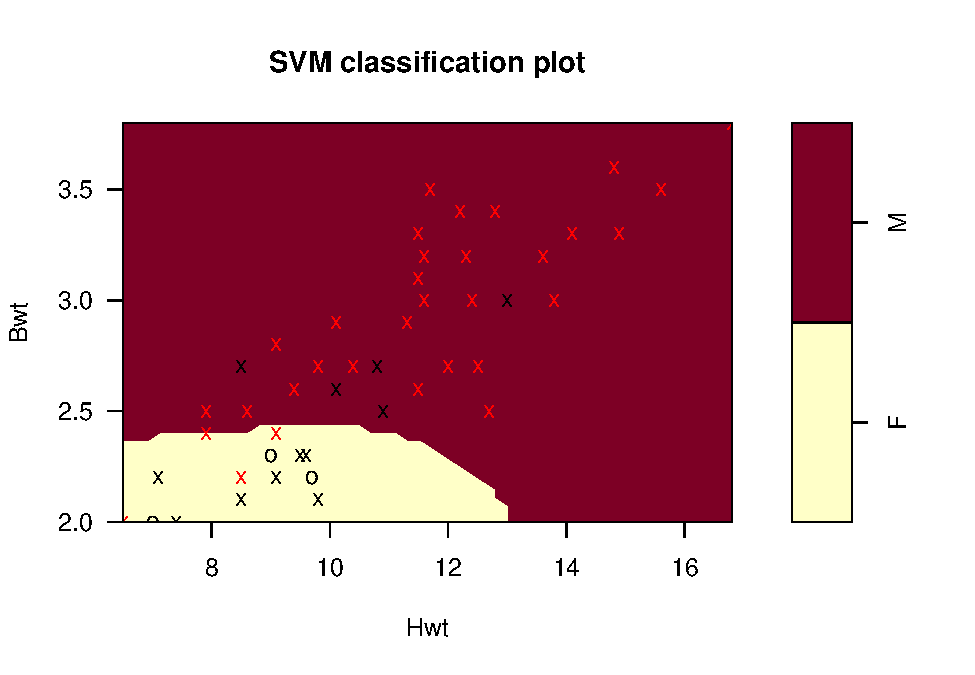
\includegraphics{R4-SA8017026_files/figure-latex/unnamed-chunk-1-1.pdf}

\hypertarget{real-data-iris}{%
\subsection{Real data: iris}\label{real-data-iris}}

First of all, for the classification problem, the `type' parameter in
the \texttt{svm()} han function has three options:
\emph{C-classification}, \emph{nu-classification}, and
\emph{one-classification}. And the `kernel' parameter has four options:
\emph{linear}, \emph{polynomial}, \emph{radial} and \emph{sigmoid}.

In order to comprehensively compare the model effects of these \emph{12}
combinations, build a self-written function

\begin{Shaded}
\begin{Highlighting}[]
\NormalTok{svm_test <-}\StringTok{ }\ControlFlowTok{function}\NormalTok{(x,y)\{}
\NormalTok{  type <-}\StringTok{ }\KeywordTok{c}\NormalTok{(}\StringTok{'C-classification'}\NormalTok{,}\StringTok{'nu-classification'}\NormalTok{,}\StringTok{'one-classification'}\NormalTok{)}
\NormalTok{  kernel <-}\StringTok{ }\KeywordTok{c}\NormalTok{(}\StringTok{'linear'}\NormalTok{,}\StringTok{'polynomial'}\NormalTok{,}\StringTok{'radial'}\NormalTok{,}\StringTok{'sigmoid'}\NormalTok{)}
\NormalTok{  pred <-}\StringTok{ }\KeywordTok{array}\NormalTok{(}\DecValTok{0}\NormalTok{, }\DataTypeTok{dim=}\KeywordTok{c}\NormalTok{(}\KeywordTok{nrow}\NormalTok{(x),}\DecValTok{3}\NormalTok{,}\DecValTok{4}\NormalTok{))}
\NormalTok{  errors <-}\StringTok{ }\KeywordTok{matrix}\NormalTok{(}\DecValTok{0}\NormalTok{,}\DecValTok{3}\NormalTok{,}\DecValTok{4}\NormalTok{)}
  \KeywordTok{dimnames}\NormalTok{(errors) <-}\StringTok{ }\KeywordTok{list}\NormalTok{(type, kernel)}
  \ControlFlowTok{for}\NormalTok{(i }\ControlFlowTok{in} \DecValTok{1}\OperatorTok{:}\DecValTok{3}\NormalTok{)\{}
    \ControlFlowTok{for}\NormalTok{(j }\ControlFlowTok{in} \DecValTok{1}\OperatorTok{:}\DecValTok{4}\NormalTok{)\{}
\NormalTok{      pred[,i,j] <-}\StringTok{ }\KeywordTok{predict}\NormalTok{(}\DataTypeTok{object =} \KeywordTok{svm}\NormalTok{(x, y, }\DataTypeTok{type =}\NormalTok{ type[i], }\DataTypeTok{kernel =}\NormalTok{ kernel[j]), }\DataTypeTok{newdata =}\NormalTok{ x)}
      \ControlFlowTok{if}\NormalTok{(i }\OperatorTok{>}\StringTok{ }\DecValTok{2}\NormalTok{) errors[i,j] <-}\StringTok{ }\KeywordTok{sum}\NormalTok{(pred[,i,j] }\OperatorTok{!=}\StringTok{ }\DecValTok{1}\NormalTok{)}
      \ControlFlowTok{else}\NormalTok{ errors[i,j] <-}\StringTok{ }\KeywordTok{sum}\NormalTok{(pred[,i,j] }\OperatorTok{!=}\StringTok{ }\KeywordTok{as.integer}\NormalTok{(y))}
\NormalTok{      \}}
\NormalTok{    \}}
  \KeywordTok{return}\NormalTok{(errors)}
\NormalTok{\}}

\NormalTok{iris_x <-}\StringTok{ }\NormalTok{iris[,}\DecValTok{1}\OperatorTok{:}\DecValTok{4}\NormalTok{]}
\NormalTok{iris_y <-}\StringTok{ }\NormalTok{iris[,}\DecValTok{5}\NormalTok{]}
\KeywordTok{svm_test}\NormalTok{(}\DataTypeTok{x=}\NormalTok{iris_x,}\DataTypeTok{y=}\NormalTok{iris_y)}
\end{Highlighting}
\end{Shaded}

\begin{verbatim}
##                    linear polynomial radial sigmoid
## C-classification        5          7      4      17
## nu-classification       5         14      5      12
## one-classification    102         75     76      75
\end{verbatim}

According to the above results, type = `C-classification' and kernel =
`radial' return the smallest amount of false positives, so this
combination can be considered to classify IRIS.

\begin{Shaded}
\begin{Highlighting}[]
\NormalTok{iris_model <-}\StringTok{ }\KeywordTok{svm}\NormalTok{(}\DataTypeTok{x=}\NormalTok{iris[,}\DecValTok{1}\OperatorTok{:}\DecValTok{4}\NormalTok{],}\DataTypeTok{y=}\NormalTok{iris[,}\DecValTok{5}\NormalTok{],}\DataTypeTok{type =} \StringTok{'C-classification'}\NormalTok{, }\DataTypeTok{kernel =} \StringTok{'radial'}\NormalTok{)}
\NormalTok{iris_pred <-}\StringTok{ }\KeywordTok{predict}\NormalTok{(}\DataTypeTok{object =}\NormalTok{ iris_model, }\DataTypeTok{newdata =}\NormalTok{ iris[,}\DecValTok{1}\OperatorTok{:}\DecValTok{4}\NormalTok{])}
\NormalTok{iris_Freq <-}\StringTok{ }\KeywordTok{table}\NormalTok{(iris[,}\DecValTok{5}\NormalTok{], iris_pred)}
\KeywordTok{print}\NormalTok{(iris_Freq)}
\end{Highlighting}
\end{Shaded}

\begin{verbatim}
##             iris_pred
##              setosa versicolor virginica
##   setosa         50          0         0
##   versicolor      0         48         2
##   virginica       0          2        48
\end{verbatim}

In this way, we saw that the correct classification rate reached
\(97.3\%\), and \(4\) samples were misjudged. In order to further
improve the classification effect, we can use the \texttt{tune.svm()}
function to find the optimal parameters of the \texttt{svm()} function.

\end{document}
